\documentclass{article}
\usepackage{amsmath}
\usepackage{graphicx}
\usepackage{listings}

\begin{document}


\section*{PROBLEM STATEMENT}
To implement the Digital Differential Analyzer (DDA) Line Drawing Algorithm in C using OpenGL, and to draw a line between two points on a 2D plane. The program will also draw the coordinate axes to visualize the line in the context of a Cartesian coordinate system.

\section*{THEORY}
The Digital Differential Analyzer (DDA) algorithm is a simple and efficient algorithm for drawing lines on raster displays. It works by calculating the intermediate points along the line based on the difference between the start and end points. The DDA algorithm incrementally plots points along the line by adding a fixed amount to the x and y coordinates at each step, which is determined by the slope of the line.

The DDA algorithm can handle any slope and ensures that the line is continuous and visually accurate. The steps are based on the larger difference between the x and y coordinates, ensuring the line is rendered correctly.

\section*{ALGORITHM}
\begin{enumerate}
    \item \textbf{Initialize}:
    \begin{itemize}
        \item Start with the initial point $(x_{start}, y_{start})$.
        \item Calculate the differences: $\text{dx} = x_{end} - x_{start}$ and $\text{dy} = y_{end} - y_{start}$.
        \item Determine the number of steps: $\text{steps} = \max(|\text{dx}|, |\text{dy}|)$.
        \item Calculate the increments: $\text{xIncrement} = \frac{\text{dx}}{\text{steps}}$ and $\text{yIncrement} = \frac{\text{dy}}{\text{steps}}$.
    \end{itemize}
    \item \textbf{Plotting}:
    \begin{itemize}
        \item Initialize the current point: $(x, y) = (x_{start}, y_{start})$.
        \item Plot the current point.
        \item For each step, update the point: $x += xIncrement$ and $y += yIncrement$, then plot the new point.
    \end{itemize}
    \item \textbf{Termination}:
    \begin{itemize}
        \item The loop terminates after all steps are completed.
    \end{itemize}
\end{enumerate}

\section*{FLOWCHART}
\begin{center}
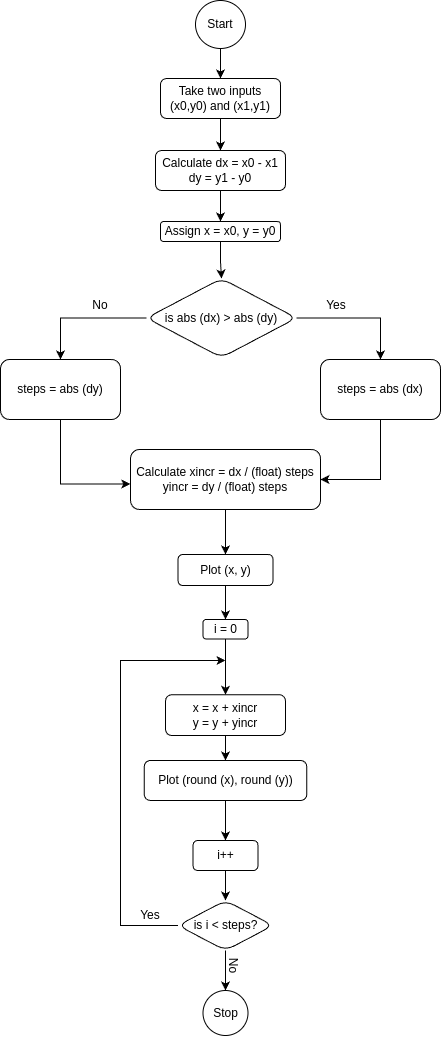
\includegraphics[width=0.7\textwidth]{flowchart.png}
\end{center}

\section*{SAMPLE I/O}
\textbf{Input:}
\begin{verbatim}
Enter the coordinates of the first point (x_start, y_start): -50 -50
Enter the coordinates of the second point (x_end, y_end): 50 50
\end{verbatim}

\textbf{Output:}
A line is drawn from $(-50, -50)$ to $(50, 50)$ on a window with coordinate axes displayed.

\section*{DISCUSSIONS}
\begin{itemize}
    \item \textbf{Accuracy}: The DDA algorithm provides accurate and visually continuous lines by incrementally plotting points based on the line's slope.
    \item \textbf{Efficiency}: While not as efficient as Bresenham's algorithm due to floating-point operations, DDA is simple to implement and understand.
    \item \textbf{Applications}: The DDA algorithm is used in various applications where line drawing is required, such as computer graphics, game development, and CAD software.
\end{itemize}

\section*{CONCLUSION}
The Digital Differential Analyzer (DDA) Line Drawing Algorithm is an effective method for rendering lines on raster displays. By incrementally plotting points based on the line's slope, the DDA algorithm ensures accurate and visually continuous lines. The implementation using OpenGL demonstrates the algorithm's capability to draw lines between any two points and visualize the coordinate axes.

\section*{CODE LISTING}
\begin{lstlisting}[language=C]
#include <GL/glut.h>
#include <stdlib.h>
#include <stdio.h>
#include <math.h>

float x_start, y_start, x_end, y_end;

void init(void)
{
    glClearColor(0.0, 0.0, 0.0, 0.0);
    glMatrixMode(GL_PROJECTION);
    gluOrtho2D(-320.0, 320.0, -240.0, 240.0);
}

void setPixel(int x, int y)
{
    glBegin(GL_POINTS);
    glVertex2i(x, y);
    glEnd();
    glFlush();
}

void drawLineDDA(float x_start, float y_start, float x_end, float y_end)
{
    float dx = x_end - x_start;
    float dy = y_end - y_start;
    float steps;
    float xIncrement, yIncrement;
    float x = x_start;
    float y = y_start;

    if (abs(dx) > abs(dy))
    {
        steps = abs(dx);
    }
    else
    {
        steps = abs(dy);
    }

    xIncrement = dx / steps;
    yIncrement = dy / steps;

    setPixel(round(x), round(y));

    for (int k = 0; k < steps; k++)
    {
        x += xIncrement;
        y += yIncrement;
        setPixel(round(x), round(y));
    }
}

void drawAxes(void)
{
    glColor3f(1.0, 1.0, 1.0);
    drawLineDDA(-320, 0, 320, 0);
    glColor3f(1.0, 1.0, 1.0);
    drawLineDDA(0, -240, 0, 240);
}

void display(void)
{
    glClear(GL_COLOR_BUFFER_BIT);
    drawAxes();
    glColor3f(0.0, 0.0, 1.0);
    drawLineDDA(x_start, y_start, x_end, y_end);
    glFlush();
}

int main(int argc, char **argv)
{
    printf("Enter the coordinates of the first point (x_start, y_start): ");
    scanf("%f %f", &x_start, &y_start);
    printf("Enter the coordinates of the second point (x_end, y_end): ");
    scanf("%f %f", &x_end, &y_end);

    glutInit(&argc, argv);
    glutInitDisplayMode(GLUT_SINGLE | GLUT_RGB);
    glutInitWindowSize(640, 480);
    glutInitWindowPosition(100, 100);
    glutCreateWindow("DDA Line Drawing Algorithm with Colored Axes");
    init();
    glutDisplayFunc(display);
    glutMainLoop();

    return 0;
}
\end{lstlisting}

\end{document}
